% -*- root: Main.tex -*-
\section{Regression}
% \subsection*{Linear Regression}
% \item{\textbf{Linear Regression:}}
\textbf{Linear Regression: } 
$RSS(\beta) = \sum_{i=1}^{n}(y_i - x_i^T\beta)^2 = (y-X\beta)^T(y-X\beta) \Rightarrow \hat{\beta} = (X^TX)^{-1}X^Ty$ \\
Prove $\hat{\beta}$ is unbiased:
$\hat{\theta} := a^T \hat{\beta}$, $\mathbb{E}_{\epsilon}[\hat{\theta}] = \mathbb{E}_{\epsilon}[a^T(X^TX)^{-1}X^Ty] = a^T(X^TX)^{-1}X^T\mathbb{E}_{\epsilon}[y] = a^T(X^TX)^{-1}X^T(X\beta + \mathbb{E}_{\epsilon}[\epsilon]) = a^T \beta$ \\
% $Var(a^T\hat{\beta}) = Var(a^T(X^TX)^{-1}X^T(X\beta + \epsilon)) = Var(a^T(X^TX)^{-1}X^T\epsilon) = \mathbb{E}(a^T(X^TX)^{-1}X^T\epsilon\epsilon^TX^(X^TX)^{-1}a) = \sigma^2a^T(X^TX)^{-1}a$ \\
Alternative unbiased estimator: $\tilde{\theta} = c^Ty = a^T\hat{\beta} + a^TDy = a^T\beta + a^TDX\beta = a^T\beta$; $a^TDX = 0$
\\
% \subsection*{Gauss Markov Theorem}
% \item{\textbf{Gauss Markov Theorem:}}
\textbf{Gauss Markov Theorem: } 
$\forall \tilde{\theta} = c^Ty$ unbiased for $a^T\hat{\beta}, \mathbb{V}(a^T\hat{\beta}) \leq \mathbb{V} (c^Ty)$; Proof: $\mathbb{V}(c^Ty) = \mathbb{E}[(c^Ty)^2] - \mathbb{E}[c^Ty]^2 = c^T(\mathbb{E}[yy^T] - \mathbb{E}[y]\mathbb{E}[y]^T)c = \sigma^2 c^Tc = \sigma^2(a^T(X^TX)^{-1}a + a^TDD^Ta) = \mathbb{V}(a^T\hat{\beta}) + \sigma^2a^TDD^Ta$
\\
% \subsection*{Bias-variance Tradeoff}
% \item{\textbf{Bias-variance Tradeoff:}}
\textbf{Bias-variance Tradeoff: } 
$\mathbb{E}_D \mathbb{E}_{Y|X=x}(\hat{f}(x) - Y)^2 = \mathbb{E}_D (\hat{f}(x) - \mathbb{E}(Y|X=x))^2 + \mathbb{E}(Y - \mathbb{E}(Y|X=x))^2 = \mathbb{E}_D (\hat{f}(x) - \mathbb{E}_D \hat{f}(x))^2 + (\mathbb{E}_D\hat{f}(x) - \mathbb{E}(Y|X=x))^2 + \mathbb{E}(Y-\mathbb{E}(Y|X=x))^2$ = \textcolor{red}{var + bias$\color{red}{^2}$ + noise}
% 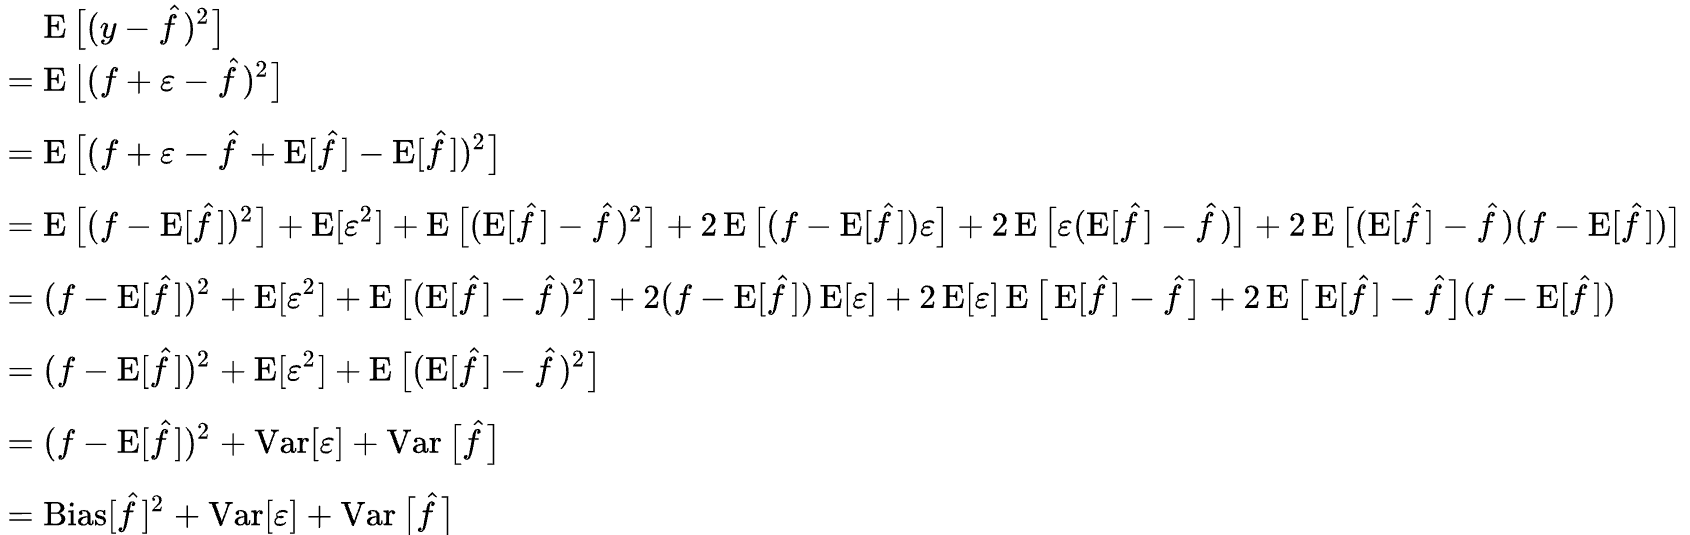
\includegraphics[scale=0.25]{b-v-tradeoff.png}
\\
% \subsection*{Regularization}
% \item{\textbf{Regularization:}}
\textbf{Regularization: } 
Can be viewed as MAP estimation with a prior. Ridge: $\beta \sim \mathcal{N}(0, \frac{\sigma^2}{\lambda I})$; Lasso: $p(\beta_i) = \frac{\lambda}{4 \sigma^2}exp(-|\beta|\frac{\lambda}{2\sigma^2})$ (Laplace, no closed-form solution since $l_1$ norm is not differentiable, more sparse estimations since the gradient of regularization does not shrink as Ridge)
\\
\textbf{Bayesian LR: } 
% \subsection*{Bayesian LR}
% \item{\textbf{Bayesian LR:}}
Assume $\epsilon \sim \mathcal{N}(0, \sigma^2 I)$, $\beta \sim \mathcal{N}(0, \wedge^{-1})$, $p(\beta|Y,X,\sigma^2, \wedge) = \mathcal{N}((X^TX+\sigma^2\wedge)^{-1}X^TY, \sigma^2(X^TX+\sigma^2 \wedge)^{-1})$ \\
Bayesian LR is a special case of Gaussian Processes with linear kernel $k(x, x') = x^T\wedge^{-1} x'$